
%%%%%%%%%%%%%%%
%	Ch7 : Compressible Flows	 %
%%%%%%%%%%%%%%%

\chapter{Quasi One-dimensional Steady Compressible flows}

\section{Total (or Stagnation) variables}

We consider the flow to be quasi one-dimensional, meaning that we suppose the variation of the section to be sufficiently slow so that we can make the approximation that the flow variables (velocity and thermodynamic variables) are uniform throughout the section, and so, only depend on x.
\\

The stagnation (or total) state is an hypothetical state where the fluid is at rest. The fluid is assumed to have been brought to rest through a steady open state reversible process without heat or work exchange. We consider a fictitious device that brings the fluid from a point $p, \rho,u$ to rest at a point $p_0, \rho_0, u_0=0$.vBy applying balance equations to this device, we get:
\\

\textbf{First principle} (where we neglect the potential energy)\textbf{:}
\begin{equation}
\begin{aligned}
&\dot{m}[(h+\frac{u^2}{2})_{out}-(h+\frac{u^2}{2})_{in}]=0 \\
\Leftrightarrow \qquad&\dot{m}[(h^0+\frac{\overbrace{u_0^2}^{u_0=0}}{2})_{out}-(h+\frac{u^2}{2})_{in}]=0 \\
\Leftrightarrow \qquad &h^0=h+\frac{u^2}{2} \equiv Stagnation \ enthalphy
\end{aligned}
\end{equation}

\textbf{Second principle:} 
\begin{equation}
\begin{aligned}
&\dot{m} [s_{out}-s_{in}]=0 \\
\Leftrightarrow \qquad &\dot{m} (s^{0}-s)=0 \\
\Leftrightarrow \qquad &s^{0}=s \equiv Stagnation \ Entropy
\end{aligned}
\end{equation}

There is no heat exchange so no reversible entropy varation and the process is assumed to be reversible so no irreversible entropy variation. Those results are shown on the Mollier diagram below.

\begin{figure}[H]
\begin{center}
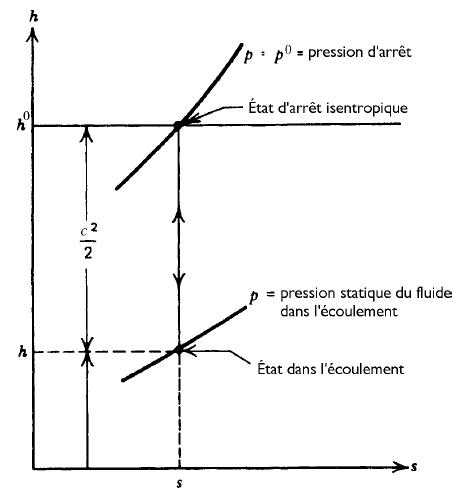
\includegraphics[scale=0.30]{ch7/chap71.png}
\caption*{Figure 7.1}
\end{center}
\end{figure}

\textbf{Bernouilli (for incompressible steady inviscid flow without body forces):}

\begin{equation}
\begin{aligned}
p+\rho \frac{u^2}{2} +\overbrace{\rho gz}^{=0 (no\ body\ forces)} =c^{st} \ along \ streamlines=p_t=p^0
\end{aligned}
\end{equation}
$p^0$ it's the pressure at a hypothetical point where the velocity would be zero. It's possible to create that hypothetical point by putting an obstacle in the flow.
\\

\textbf{For compressible flow:}

\begin{equation}
\left\{
    \begin{array}{ll}
    h^0=h+\frac{u^2}{2}  \\
    s^0=s
    \end{array}
\right.
\end{equation}

\begin{equation}
Mach\ number: M=\frac{u}{a}
\end{equation}
\begin{equation}
For\ a\ calorically\ perfect\ gas: h=C_pT=\frac{C_p}{R}RT=\frac{\gamma}{\gamma-1}\frac{p}{\rho}=\frac{a^2}{\gamma -1} 
\end{equation}
\begin{equation}
Speed\ of\ sound: a^2=\frac{\partial p}{\partial \rho}|_s \ \rightarrow for\ a\ perfect\ gas:\ a^2=\gamma \frac{p}{\rho}=\gamma RT
\end{equation}

\begin{equation}
 h^0=h+\frac{u^2}{2} \Leftrightarrow h^0=h(1+\frac{u^2}{2h}) \Leftrightarrow h^0=h(1+\frac{u^2}{2} \frac{\gamma -1}{a^2}) \\
 \Leftrightarrow h^0=h(1+ \frac{\gamma -1}{2} M^2) 
\end{equation}
\\

For an isentropic evolution ($pv^k=c^{st}$) of a calorically and hydraulically perfect gas:
\begin{equation}
\begin{aligned}
\frac{p}{\rho}=(\frac{T^0}{T})^{\gamma/\gamma-1}=(\frac{h^0}{h})^{\gamma/\gamma-1} \\
\Leftrightarrow \frac{p^0}{p}=(1+\frac{\gamma-1}{2}M^2)^{\gamma/\gamma-1} \\
\Leftrightarrow p^0=p(1+\frac{\gamma-1}{2}M^2)^{\gamma/\gamma-1}\ (1)
\end{aligned}
\end{equation}
\\

\textbf{For incompressible flow:}
\begin{equation}
\begin{aligned}
\underbrace{p^0}_{Stagnation\ pressure}=\underbrace{p}_{Static\ pressure}+\underbrace{\rho\frac{u^2}{2}}_{Dynamic\ pressure} \ (2)
\end{aligned}
\end{equation}

So now, what we want to do is compare (1) and (2). We know that for small Mach number, we get an incompressible flow. As a matter of fact, we have seen that when M is small we can make the approximation of constant density (Remember the relation: $-M^2\frac{du}{u}=\frac{d\rho}{\rho}$). So what we want is to make an expansion of (1) for low Mach number.

\begin{equation}
\begin{aligned}
&By\ applying\ the\ binomial\ formula\ to\ (1): (1+\epsilon)^m=1+m\epsilon+m\frac{m-1}{2} \epsilon^2+... \\
&Where\ \epsilon=\frac{\gamma-1}{2}M^2\ and\ m=\frac{\gamma}{\gamma-1},\ we\ get:\\
&\ p^0=p[1+\frac{\gamma}{\gamma-1}\frac{\gamma-1}{2}M^2]+\frac{\gamma}{\gamma-1}\frac{\frac{\gamma}{\gamma-1}-1}{2}(\frac{\gamma-1}{2}M^2)^2+...] \\
& p^0=p+\underbrace{ \gamma \frac{M^2}{2}p}_{=\gamma \frac{p}{2}\frac{u^2}{a^2}=\rho \frac{u^2}{2}}+\gamma \frac{M^4}{8}p+...
\end{aligned}
\end{equation}

We see that the two first term (in this expansion of the equation for compressible flow) are exactly the same as the one from the Bernouilli equation for incompressible flow!

\section{Conservation equation for steady quasi 1D compressible flows}

We consider a piece of duct with slow cross sectionnal area variation A(x). We are going to make balance over an infinitesimal slice dx.  We make the quasi one-dimensional assuptions that tells us that the flow quantities are uniform in each sections (flow quantities only dependant on x). Note that this is an approximation. It doesn't take into account viscosity. Velocity is not purely axial so we consider here that the velocity components are negligeable towards the axial velocity components.
\begin{equation}
\left\{
    \begin{array}{ll}
    \vec{u}=u(x)\vec{e_x} \\
    p=p(x) \\
    \rho=\rho(x)
    \end{array}
\right.
\end{equation}

\begin{figure}[H]
\centering
\begin{minipage}{.5\textwidth}
  \centering
  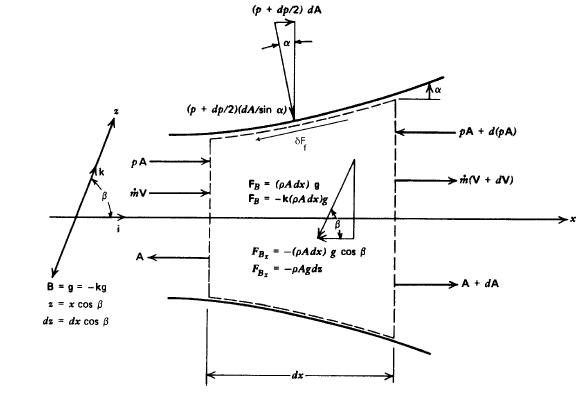
\includegraphics[scale=0.30]{ch7/chap72.png}
  \caption*{Figure 7.2}
  \label{fig:test1}
\end{minipage}%
\begin{minipage}{.5\textwidth}
  \centering
  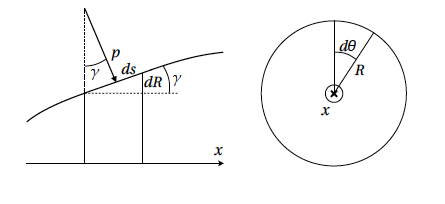
\includegraphics[scale=0.30]{ch7/chap73.png}
  \caption*{Figure 7.3}
  \label{fig:test2}
\end{minipage}
\end{figure}

\textbf{Mass balance:} 

\begin{equation}
\begin{aligned}
&\underbrace{Rate\ of\ accumulation}_{=0\ steady\ flow}+Net\ mass\ flow\ out=\underbrace{Production\ of\ mass}_{=0\ no\ mass\ production} \\
&\Leftrightarrow Net\ mass\ flow\ out=0 \Leftrightarrow \dot{m_E}-\dot{m_W}=0 \Leftrightarrow \rho u A|_{x+dx}-\rho u A|_{x}=0 \Leftrightarrow d(\rho u A)=0 \\
&By\ dividing\ by\ \rho u A,\ we\ get\ : \frac{d \rho}{\rho}+\frac{du}{u}+\frac{dA}{A}=0
\end{aligned}
\end{equation}

\textbf{Axial momentum balance:} 

\begin{equation}
\begin{aligned}
&\underbrace{\dot{m}_{x+dx}u(x+dx)-\dot{m}_{x}u(x)}_{net\ momentum\ flow\ out}=\rho u Adu\ (because\ \dot{m}_{x+dx}=\dot{m}_{x})\\
=&\overbrace{\underbrace{(pA)_x}_{contribution\ of\ West}-\underbrace{(pA)_{x+dx}}_{contribution\ of\ East}}^{=-d(pA)} -\tau_w P_{er} dx -\rho A \underbrace{dx cos\phi}_{=dz} g\\
&+\underbrace{pdA}_{=pressure\ force\ on\ the\ side\ walls}
\end{aligned}
\end{equation}

Note: To find the pressure force on the side walls we magnified an element dx, for which we found $pdSP_{er}sin \gamma \ where\  dS sin \gamma=dR \Leftrightarrow p2 \pi RdR=pd(\pi R^2)=pdA$ (cf. figure 7.3).

So we have:
\begin{equation}
\begin{aligned}
\rho u Adu=\underbrace{-d(pA)+pdA}_{=-Adp}-\rho Agdz- \tau_w P_{er} dx \\
\end{aligned}
\end{equation}

Dividing by $\rho A$, we get:
\begin{equation}
\begin{aligned}
udu=-\frac{d\rho}{\rho}-gdz-\frac{\tau_w}{\rho} \frac{P_{er}}{A}dx
\end{aligned}
\end{equation}

Remebering that $\tau_w=\frac{C_f}{\frac{\rho u^2}{2}}$ and by using the definition of the hydraulic diameter $D_h=\frac{4A}{P_{er}}$, we get:
\begin{equation}
\begin{aligned}
udu+\frac{d\rho}{\rho}+gdz&=-C_f \frac{u^2}{2} \frac{4}{D_h}dx
\\
&= -\frac{u^2}{2} \underbrace{4C_f  \frac{dx}{D_h}}_{\equiv \delta f=friction\ (dimensionnless\ and\ infinitesimal)}
\end{aligned} 
\end{equation}

\textbf{Energy balance (First principle):}
\\

The rate of change of energy (=0 here because steady flow)+total energy flow=rate of change brought to the system which is mechnaical power and heat:
\begin{equation}
\begin{aligned}
\underbrace{\dot{m}}_{=\rho u A} d(h+\frac{u^2}{2})=\delta \dot{W} +\delta \dot{Q}
\end{aligned} 
\end{equation}
Where $\delta \dot{W}=0$ because there is no mechanical power exchange (no turbine or pump) and $\delta \dot{Q} \neq 0$ because there is heat exchange through the walls.
\\

Note: There is no power of the pressure of the side forces because there is no velocity there.
\\

Let's now divide the equation by $\dot{m}$, we get:
\begin{equation}
\begin{aligned}
d(h+\frac{u^2}{2})=dh+udu=\delta \underbrace{\frac{\dot{Q}}{\dot{m}}}_{\equiv \delta q=heat\ energy\ p.u.\ mass} \Leftrightarrow dh+udu=\delta q 
\end{aligned} 
\end{equation}

\textbf{Second principle balance:}
\\

\begin{equation}
\begin{aligned}
&\dot{m}ds=\frac{\delta \dot{Q}}{T}+\dot{m}d \underbrace{\sigma_i}_{internal/irreversible\ entropy\ production >0 }\\
&Dividing\ by\ \dot{m},\ we\ get: ds=\frac{\delta q}{T}+\underbrace{d\sigma_i}_{>0}
\end{aligned} 
\end{equation}
\\

By putting the first principle together with the momentum balance equation (assuming no body forces) and by using Gibbs relations ($de=Tds-pdv$ and $dh=Tds+vdp$), we get:

\begin{equation}
\begin{aligned}
&\underbrace{dh-\frac{dp}{\rho}}_{=Tds\ by\ Gibbs}=\delta q+\frac{u^2}{2} \delta f  \\
Dividing\ by\ T,\ we\ get: &ds=\frac{\delta q}{T} +\frac{u^2}{2T} \underbrace{\delta f}_{>0\ because\ friction\ is\ only\ positif}
\end{aligned} 
\end{equation}

This last equation shows that the irreversible entropy production is linked to the friction ($d\sigma_i=\frac{u^2}{2T} \delta f \geq 0$). So the second principle doesn't bring any additionnal information. Therefore the flow is entirely described by the three equation: mass conservation, moementum equation and first principle.
\\

Three equations that describe the flow:
 \begin{equation}
\begin{aligned}
&1)\ \frac{d\rho}{\rho}+\frac{du}{u}=-\frac{dA}{A} \\
&2)\ udu+\frac{dp}{\rho}=-\frac{u^2}{2} \delta f\\
&3)\ dh+udu=\delta q
\end{aligned} 
\end{equation}

These equations expresses how the flow variables vary accros the slice dx. Those variables can vary accros the slice due to three possible effects: area change, friction, heat addition.
The flow inside the duct is characterized by three quantities: 2 thermodynamics $(p,\rho)$ quantities describing the state of the fluid and the velocity $(u)$ (h being a function of $p\ and\ \rho$ ($h=h(p,\rho)$). Example for a perfect gas: $h=C_pT=C_p\frac{p}{\rho R}=\frac{\gamma}{\gamma-1}\frac{p}{\rho}$.
\\

So we have three cases:
 \begin{equation}
\begin{aligned}
&1)\ dA \neq 0, \delta f=0, \delta q=0 \\
&2)\ dA=0, \delta f\neq0, \delta q=0 \\
&3)\ dA=0, \delta f=0, \delta q\neq0 \\
\end{aligned} 
\end{equation}

\section{Quasi 1D isentropic flow (nozzle) (effect of area change)}

By looking at the second principle, if $\delta f=0\ and\ \delta q=0$ we get $ds=0$ which gives (using the definition of the speed of sound $a$):
 \begin{equation}
\begin{aligned}
dp=\underbrace{\frac{\partial p}{\partial \rho}|_s}_{\equiv a^2}d\rho
\end{aligned} 
\end{equation}

The equations becomes:
 \begin{equation}
\begin{aligned}
&1)\ \frac{d\rho}{\rho}+\frac{du}{u}=-\frac{dA}{A} \\
&2)\ udu+a^2\frac{d\rho}{\rho}=0
\end{aligned} 
\end{equation}

Let's take $(2)-u^2(1)$, we get:
The equations becomes:
 \begin{equation}
\begin{aligned}
&(udu+a^2\frac{d\rho}{\rho})-u^2(\frac{d\rho}{\rho}+\frac{du}{u}+\frac{dA}{A})=0 \\
& \Leftrightarrow (a^2-u^2)\frac{d\rho}{\rho}=u^2\frac{dA}{A} \\
&by\ dividing\ by\ a^2,\ we\ get: (1-M^2)\frac{a^2d\rho}{\rho}=u^2\frac{dA}{A} \\
& \Leftrightarrow (1-M^2)\frac{dp}{\rho}=u^2\frac{dA}{A}
\end{aligned} 
\end{equation}

We end up with 2 very interesting equations (valid for any type of fluid (not only perfect gases)):
The equations becomes:
 \begin{equation}
\begin{aligned}
&1)\ (1-M^2)\frac{dp}{\rho}=u^2\frac{dA}{A} \\
&2)\ (1-M^2)udu=-u^2\frac{dA}{A}
\end{aligned} 
\end{equation}

From the second equation we can see that $du$ has the opposite sign of $dA$, so when $dA<0 \Rightarrow u \uparrow$. Let's make a table that illustrates the different variations of $p,\rho,u$ for Mach number smaller than one (subsonic flow) or bigger thant one (supersonic flow).
\\

\begin{center}
\begin{tabular}{|l|c|r|}
  \hline
   &$dA<0$ & $dA>0$ \\
   &convergent & divergent \\
  \hline
  $M<1$ & $u \uparrow, p \downarrow$ & $u \downarrow, p \uparrow$  \\
  (subsonic) & nozzle & diffuser\\
  \hline
  $M>1$ & $u \downarrow, p \uparrow$ & $u \uparrow, p \downarrow$ \\
  (supersonic) &  & \\
  \hline
\end{tabular}
\end{center}

Notes:
\begin{itemize}
\item variation of p is opposite to the variation of u, so when $u \uparrow \Rightarrow p \downarrow$
\item nozzle=expansion device and diffuser=compression device
\item The second line of the table is the opposite of the first line
\end{itemize}

When the flow is sonic ($M=1$) it implies that $dA=0$. Meaning that sonic flow conditions can only be achieved at a cross section extremum (it's actually at a minimum; the throat). This leads to the concept of saturation.
\\

Note: The flow being isentropic, if $p \downarrow$ then $T \downarrow$, then $a \downarrow$ and so $u \uparrow$ and $M \uparrow$.
\\

Saturation: There is a limit inlet velocity corresponding to sonic exit conditions. There is a limit mass flow that can be pushed trough the nozzle (cf. figure 7.4).
\\
\begin{figure}[H]
\begin{center}
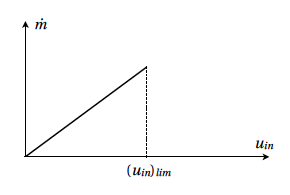
\includegraphics[scale=0.30]{ch7/chap74.png}
\caption*{Figure 7.4}
\end{center}
\end{figure}


For a perfect gas (both thermically perfect ($p=\rho RT$) and calorically perfect ($C_p and C_v \ are\ constant$)):
\begin{equation}
\left\{
    \begin{array}{l}
    a^2=\gamma RT=\gamma \frac{p}{\rho}=(\gamma -1)h \\
    h=\frac{\gamma}{\gamma-1}\frac{p}{\rho}=\frac{a^2}{\gamma-1} \\
    3^d \ equation: dh=udu=dh^0=0 \Rightarrow h^0=c^{st} \Leftrightarrow \frac{dh^0}{dx}=0
    \end{array}
\right.
\end{equation}
The last equation shows that the stagnation enthalpy remains constant along the axis of the duct.

And we know that $ds=0$ and $ds=ds^0$ (by the definition of the stagnation state) $\Rightarrow s^0=c^{st}$.

The stagnation state remains constant along the axis of the duct because $s^0 \ and\ h^0$ are constant $\Rightarrow p^0=c^{st}\  (\frac{dp^0}{dx}=0)$. Therefore the stagnation enthalpy is not a function of x because it is constant along the axis of the duct ($h^0=h+\frac{u^2}{2} \neq f(x)$).
\\

Let's rewrite the equations in another form:
 \begin{equation}
\begin{aligned}
&h^0=h+\frac{u^2}{2}  \rightarrow h(1+\frac{(\gamma-1) u^2}{2a^2})=h^0  \rightarrow h=h^0(1+\frac{(\gamma-1) }{2}M^2)^{-1} \\
& \rightarrow\frac{h}{h^0}=\frac{T}{T^0}=(1+\frac{(\gamma-1) }{2}M^2)^{-1}
\end{aligned} 
\end{equation}
The flow being isentropic we have:
 \begin{equation}
\begin{aligned}
&\frac{p}{p^0}=(\frac{T}{T^0})^{\frac{\gamma}{\gamma-1}}=(1+\frac{(\gamma-1) }{2}M^2)^{\frac{-\gamma}{\gamma-1}} \\
&\frac{\rho}{\rho^0}=\frac{p}{p^0} \div \frac{T}{T^0}=(1+\frac{(\gamma-1) }{2}M^2)^{\frac{-1}{\gamma-1}} 
\end{aligned} 
\end{equation}

\textbf{Critical flow conditions (M=1) indicated by a *:}

 \begin{equation}
\begin{aligned}
&\frac{h^*}{h^0}=(\frac{\gamma+1 }{2})^{-1} \\
&\frac{p^*}{p^0}=(\frac{\gamma+1}{2})^{\frac{-\gamma}{\gamma-1}} \\
&\frac{\rho^*}{\rho^0}=(\frac{\gamma+1}{2})^{\frac{-1}{\gamma-1}} 
\end{aligned} 
\end{equation}

By combining $h/h^0$ with $h^*/h^0$, $p/p^0$ with $p^*/p^0$ and $\rho/\rho^0$ with $\rho^*/\rho^0$, we get: 

 \begin{equation}
\begin{aligned}
&\frac{h}{h^*}=\frac{(1+\frac{(\gamma-1) }{2}M^2)^{-1}}{(\frac{\gamma+1 }{2})^{-1}}\\
&\frac{p}{p^*}= \frac{(1+\frac{(\gamma-1) }{2}M^2)^{\frac{-\gamma}{\gamma-1}}}{(\frac{\gamma+1}{2})^{\frac{-\gamma}{\gamma-1}}}\\
&\frac{\rho}{\rho^*}=\frac{(1+\frac{(\gamma-1) }{2}M^2)^{\frac{-1}{\gamma-1}} }{(\frac{\gamma+1}{2})^{\frac{-1}{\gamma-1}} }
\end{aligned} 
\end{equation}

Note:  $\frac{p^0}{p^*}=(\frac{\gamma+1}{2})^{\frac{\gamma}{\gamma-1}}$ for $\gamma=1.4$ we get: $\frac{p^0}{p^*}=1.89$. So we get sonic conditions at the outlet if $\frac{p^0}{p^*} \geq 1.89$.

\section{Flow in a nozzle of given shape (=cross sectional area distribution A(x))}

Known data: $p^0\ (reservoir\ stagnation\ pression),\ T^0,\ A(x), \ p_{ext}$.

 \begin{equation}
\begin{aligned}
&\bullet\  \frac{p}{p^0}=(1+\frac{(\gamma-1) }{2}M^2)^{\frac{-\gamma}{\gamma-1}} \rightarrow \ At\ the\ exit: 
\frac{p_{exit}}{p^0}=(1+\frac{(\gamma-1) }{2}M^2_{exit})^{\frac{-\gamma}{\gamma-1}} \\ 
& \Leftrightarrow M_{exit}=\sqrt{\frac{2}{\gamma-1}[(\frac{p^0}{p_{exit}})^{\frac{\gamma-1}{\gamma}}-1]} \\
&\bullet\ \frac{A}{A^*}=\varphi(M) \rightarrow A^*=\frac{A}{\varphi(M)}
\end{aligned} 
\end{equation}

We see that there is a condition $A^* \leq A_{throat} \Rightarrow \varphi(M{exit}) \geq \frac{A_{exit}}{A_{throat}} \Rightarrow M_{exit}\leq (M_{exit})_{max}$. $A^*$ is the minimum cross section (because the sonic cross section is the minimum crosse section). The throat area cannot be smaller that the critical one. 

This is shown in the figure 7.5 where we see that there is a minimum for $A/A^*=1$ that corresponds to $M=1$. We can also see, as seen before, that the Mach number of a subsonic flow increase in a convergent nozzle and the Mach number of a supersonic flow also increase in a divergent nozzle.
\\

When we have $A^*$, we know $A(x)$ in each section, so we can compute M, and once we have M, we can compute all quantities ($p, T,...$).
\\

If the exit pressure is equal to the stagnation pressure (which is equal to the inlet pressure for a reservoir), then there is no flow (Pressure is uniform $\rightarrow$ No flow and $\frac{p}{p^0}=0$ everywhere).

\begin{figure}[H]
\begin{center}
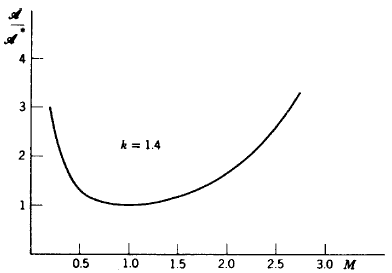
\includegraphics[scale=0.30]{ch7/chap75.png}
\caption*{Figure 7.5}
\end{center}
\end{figure}

Let's now study the flow in a nozzle of a given shape depending on the downstream pressure ($p_s$ on the figure 7.6). 

\begin{itemize}
\item If the downstream pressure is equal to the stagnation pressure ($p_s=p^0$) then the fluid is at rest (no flow).
\item If we decrease the downstream pressure, a flow is established in the nozzle. As long as the pressure ratio $p_s/p^0$ is such that the flow is subsonic at the throat ($A_s/A_{throat} < A/A^*(M_s)$), there exist a unique solution (point b in the figure 7.6).
\item When the pressure is such that $A_s/A_{throat}=A/A^*(M_s)$, the flow is sonic at the throat and subsonic (compression) in the divergent. (Note: $A_s=$downstream section). This case correspond to the point c in the figure 7.6.
\item If we continue to decrease the pressure, then there is no more isentropic solutions, except for the case $d$ in the figure that corresponds to a supersonic flow (expansion) in the divergent. In this case, we say that the nozzle is adapted.
\item For any intermediate pressure between the cases $c$ and $d$, there would be irreversible phenomena that would appear inside or outside the nozzle. (Note that for point $c$ and $d$ the mass flow is the same). For now we do not knwow what these phenomena are (we will see them later) but we know that there is no quasi 1D solutions in this interval.
\end{itemize}

\begin{figure}[H]
\begin{center}
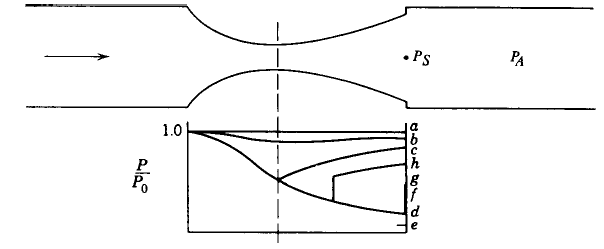
\includegraphics[scale=0.55]{ch7/chap76.png}
\caption*{Figure 7.6}
\end{center}
\end{figure}

\section{Flow with friction (no area variation and no heat exchange)}

Our equations becomes:
 \begin{equation}
\begin{aligned}
&1)\ \frac{d\rho}{\rho}+\frac{du}{u}=-\frac{dA}{A}=0 \Rightarrow d(\rho u)=0 \Rightarrow \rho u=c^{st} \equiv G \Rightarrow u=Gv \\
&2)\ \frac{dp}{\rho}+udu=\frac{-u^2}{2} \delta f \ (where \ \delta f =4C_f\frac{dx}{D_h} ) \\
&3)\ dh+udu=\delta q=0 \\
& Gibbs: dh=Tds-\frac{dp}{\rho}
\end{aligned} 
\end{equation}
Using 2, 3 and Gibbs, we get ($\delta q$= reversible entropy increase and $\delta f$= irreversible entropy increase):
 \begin{equation}
\begin{aligned}
&Tds=\underbrace{\delta q}_{=0}+\frac{u^2}{2}\delta f \rightarrow ds^0=ds \neq 0 \Rightarrow dp^0 \neq 0 \\
&By\ the\ second\ principle: dp^0<0\quad because\ ds^0>0
\end{aligned} 
\end{equation}
Finally, the equation 3, can be rewriten as:
 \begin{equation}
\begin{aligned}
&d \underbrace{(h+\frac{u^2}{2})}_{\equiv h^0}=dh^0=0 \rightarrow h^0(x)=c^{st} (\Leftrightarrow \frac{dh^0}{dx}=0) \\
& \rightarrow h+\frac{u^2}{2}=c^{st} \rightarrow h+\frac{G^2v^2}{2}=h^0 \ Fanno\ Line\ equation
\end{aligned} 
\end{equation}
States along the flow are defined by this last equation (Fanno line equation) which contains only thermodynamics quantities. This equation is represented in the Mollier diagram in figure 7.7.

\begin{figure}[H]
\begin{center}
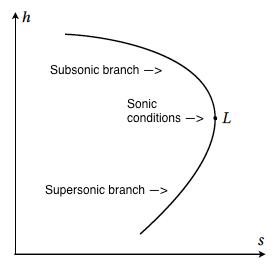
\includegraphics[scale=0.45]{ch7/chap77.png}
\caption*{Figure 7.7}
\end{center}
\end{figure}

Notes on figure 7.7:
\begin{itemize}
\item Subsonic branch: friction accelerates the flow: $p \downarrow, u\uparrow$.
\item Supersonic branch: friction decelarates the flow.
\item At L, we reach sonic conditions. We see that this is a limit. There is a saturation like there was for area change. There is a maximum mass flow rate that can be pushed inside a duct of a certain lenght. There is a maximum length ($L_{max}$) meaning that if the conisdered duct is longer than this maximum length the inlet condtions are not realizable, specifically that the mass flow is too high. There is a maximum value for friction. The pressure in the duct cannot go below $p_L$ (meaning that the velicty cannot go beyond $u_L$).
\item The entropy increases along the pipe because of the irreversibility brought by the friction. At point L we see that ds=0 (vertical tangent), therefore $\delta f=0$ and $u^2=a^2$ meaning that $M=1$ (sonic conditions). We see that it is impossible to get supersonic with friction, as if the inlet velocity is supersonic, the friction wil lower the velocity.
\item For a fluid entering with subsonic conditions, friction will have for effect to decrease the pressure which will lead to a decrease of density and so to an increase of velocity and a decrease of enthalpy.
\item As mentionned, the inferior branch of the Fanno Line correspond to supersonic inlet conditions. In thoses cases, friction has for effect (paradoxally) to compress the fluid. The reason is that the head loss has for main effect to reduce the speed, which leads to an increase of density (by mass conservation) and an increase of pressure. We see that friction has for effect to make the Mach number tend to one (same as the convergence of a nozzle).
\end{itemize}

Let's now see some mathematical expressions for a perfect gas (Note: since $p^0$ is not a constant we are going to use the critical conditions that are always unique and are never dependent on w and on the type of flow):

Using:
 \begin{equation}
\begin{aligned}
&h+\frac{u^2}{2}=h^0=c^{st} \\
&\frac{h^0}{h}=1+\frac{\gamma-1}{2}M^2 \\
&\frac{h^*}{h^0}=\frac{1}{\frac{\gamma +1}{2}}\\
&M=\frac{u}{a} 
\end{aligned} 
\end{equation}
We get:
 \begin{equation}
\begin{aligned}
&\frac{h}{h^*}=\frac{\frac{\gamma+1}{2}}{1+\frac{\gamma-1}{2}M^2} =\frac{T}{T^*}=\frac{a^2}{a^*} \\
&u=Ma \rightarrow \frac{u}{a^*}=M\frac{a}{a^*}=M[\frac{\frac{\gamma+1}{2}}{1+\frac{\gamma-1}{2}M^2}]^{1/2} \\
& \rho u=\rho^* a^*\ (by\ mass\ conservation)\ \rightarrow \frac{\rho}{\rho^*}=\frac{a^*}{u}=\frac{1}{M} [\frac{\frac{\gamma+1}{2}}{1+\frac{\gamma-1}{2}M^2}]^{-1/2} \rightarrow \frac{p}{p^*}=\frac{\rho}{\rho^*}\frac{T}{T^*}
\end{aligned} 
\end{equation}
Finally, since we talked about it, it is interesting to know that the maximmum lenght of the duct $L_{max}$ can be derived from our 3 equations: $dh+udu=0, \frac{d\rho}{\rho}+\frac{du}{u}=0 \ and\ udu+\frac{dp}{\rho}=\frac{-u^2}{2} \delta f$:

 \begin{equation}
\begin{aligned}
\frac{4fL_{max}}{D_h}=\frac{1-M^2}{\gamma M^2}+\frac{\gamma+1}{2\gamma}ln(\frac{\frac{\gamma+1}{2}M^2}{1+\frac{\gamma-1}{2}M^2} ) \ with\ \delta f=\frac{4f dx}{D_h}
\end{aligned} 
\end{equation}

\section{Flow with heat exchange (no area variation and no friction)}

Our equations becomes:
 \begin{equation}
\begin{aligned}
&1)\ \frac{d\rho}{\rho}+\frac{du}{u}=-\frac{dA}{A}=0 \Rightarrow d(\rho u)=0 \Rightarrow \rho u=c^{st} \equiv G \Rightarrow u=Gv \\
&2)\ \frac{dp}{\rho}+udu=\frac{-u^2}{2} \delta f=0 \ (where \ \delta f =4C_f\frac{dx}{D_h} ) \\
&3)\ dh+udu=\delta q \neq 0 \rightarrow dh^0=dh+udu \neq 0 \Rightarrow h^0(x) \neq c^{st}
\end{aligned} 
\end{equation}
From which, we can find:
 \begin{equation}
\begin{aligned}
&\frac{dp}{\rho}+udu=\frac{-u^2}{2} \delta f=0 \rightarrow dp+\underbrace{\rho u}_{=G}du=0  \Leftrightarrow p+Gu=c^{st} \\ 
&\Leftrightarrow p+G^2v=c^{st} \ Rayleigh\ Line\ equation
\end{aligned} 
\end{equation}
States along the flow are defined by this last equation (Rayleigh line equation) which contains only thermodynamics quantities. This equation is represented in the Mollier diagram in figure 7.8.

\begin{figure}[H]
\begin{center}
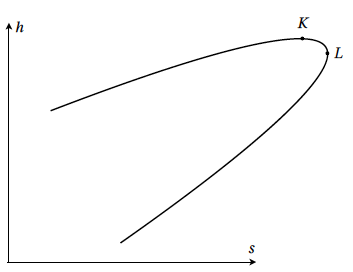
\includegraphics[scale=0.45]{ch7/chap78.png}
\caption*{Figure 7.8}
\end{center}
\end{figure}
Notes on figure 7.8:
\begin{itemize}
\item K: maximum of enthalpy beyond which the addition of heat make the kinetic energy increase and the temperature decrease.
\item L: maximum of entropy which leads to a point of thermal saturation, corresponding to the maximum heat that can be added to the system
\item $\delta q$ can be $>0\ or\ <0$ (heat can be added but also remove from the system)
\item For a fluid entering the duct with subsonic conditions, the addition of heat will be expressed by an augmentation of entropy (reversible transformation), which is accompanied by a diminution of pressure and density and therfore by an increase of velocity.
\item As mentionned, we see two interesting points. A maximum of enthalphy (K) and a maximum of entropy (L). Initially, the addition of heat is accompanied by an augmentation of enthalpy, until the point K from where the addition of heat transforms integrally in kinetic energy. Beyond K, the addition of kinetic energy is superior than the addition of heat which brings a diminution of enthalphy. As for the maximum of entropy, it indicates, once again, the phenomenon of saturation. Indeed, it results from it that the quantity of heat brought to the fluid is bounded above by the quantity of heat bringing him to the state L. In this case we talk about thermal saturation.
\item In the superior part of the Rayleigh line (which corresponds to a subsonic flow), the addition of heat has for effect to accelerate the fluid to sonic conditions. On the contrary, in the inferior part of the Rayleigh line (which corresponds to a supersonic flow), the addition of heat has for effect to decelerate the fluid to sonic conditions (same effect as a diminution of section). 
\\

\end{itemize}

The point L corresponds to $ds=0$ so $\delta q=0$ and as $dp=a^2d\rho$ we have: $a^2\frac{d\rho}{\rho}+udu=0$ and as  $\frac{d\rho}{\rho}+\frac{du}{u}=0$ we get: $u^2=a^2 \Leftrightarrow M=1$. Which shows that the critical conditions at L corresponds to the sonic conditions.
\\

For perfect gases:
 \begin{equation}
\begin{aligned}
& G=\rho u \rightarrow G^2=\rho^2 u^2=\rho^2 M^2 \underbrace{a^2}_{a^2=\frac{\gamma p}{\rho}} =M^2 \rho \gamma p \rightarrow G^2v=\gamma M^2p \\ 
&p+\underbrace{G^2v}_{=\gamma M^2p}=p^*+G^2v^* \rightarrow (1+\gamma M^2)p=(1+\gamma)p^*
 \rightarrow \frac{p}{p^*}=\frac{1+ \gamma
 }{1+ \gamma M^2}
\end{aligned} 
\end{equation}
Finally, by mass conservation (remember that by definition $u=a^*$ at critical conditions):
 \begin{equation}
\begin{aligned}
&\rho u=\rho^* a^* \rightarrow \rho M a=\rho^* a^* \rightarrow \frac{Mp}{RT} \sqrt{\gamma RT}=\frac{p^*}{RT^*}\sqrt{\gamma RT^*} \\
& \sqrt{\frac{T}{T^*}}=M\frac{p^*}{p} \rightarrow \frac{T}{T^*}=M^2(\frac{1+\gamma}{1+\gamma M^2})^2
\end{aligned} 
\end{equation}

\section{Normal shockwave}

\begin{figure}[H]
\centering
\begin{minipage}{.5\textwidth}
  \centering
  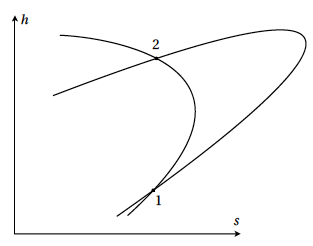
\includegraphics[scale=0.40]{ch7/chap791.png}
  \caption*{Figure 7.9}
  \label{fig:test1}
\end{minipage}%
\begin{minipage}{.5\textwidth}
  \centering
  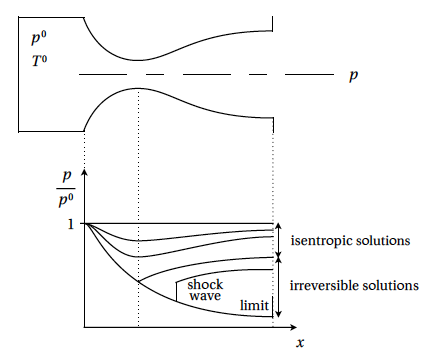
\includegraphics[scale=0.40]{ch7/chap792.png}
  \caption*{Figure 7.10}
  \label{fig:test2}
\end{minipage}
\end{figure}

If we put on the same Mollier diagram a Fanno line and a Rayleigh line (for the same mass flow), we see that they intersect in two points. One corresponding to a supersonic flow (1) and one to subsonic flow (2). We conclude that a spontaneous jump from 1 to 2, without heat exchange (by definition of the Fanno line) and without friction (by definition of the Rayleigh line) is possible. Such a sudden change (discontinuity) is called a shock wave. We see that it is a compression wave since $p_2>p_1$ ($u_2<u_1$). This result is shown on figure 7.9.
\\

Note that we can jump from 1 to 2 because it respects the second principle ($ s_2>s_1 $). In the contrary a jump from 2 to 1 is impossible since it would mean decrease of entropy. Since $ s_2>s_1$ and the transformation is adiabatic (by definition of the Fanno line) we conclude that the shock wave is an irreversible phenomenon.

The relations between 1 and 2 are called the jump conditions or Rankine-Hugoniot equations. Those equations are obtained applying our 3 famous equations to this situation:

 \begin{equation}
\begin{aligned}
&1)\ Mass: \rho_2 u_2=\rho_1 u_1 \ (no\ area\ change) \\
&2)\ Momentum: \rho_2 u_2^2-\rho_1 u_1^2=p_1-p_2 \Leftrightarrow p_2+\rho_2 u_2^2=p_1+\rho_1 u_1^2\ (no\ friction)\\
&3)\ First\ principle: h_2+\frac{u_2^2}{2}=h_1+\frac{u_1^2}{2} \ (no\ heat\ transfer)
\end{aligned} 
\end{equation}

Let's eliminate the velocities :
 \begin{equation}
\begin{aligned}
&From\ 1\ we\ get:u_2=\frac{\rho_1}{\rho_2}u_1\ that\ we\ put\ in\ 2: p_2+\rho_2 (\frac{\rho_1}{\rho_2}u_1)^2=p_1+\rho_1 u_1^2 \\
& \Leftrightarrow p_2-p_1=u_1^2(\rho_1-\rho_2(\frac{\rho_1}{\rho_2})^2) \Leftrightarrow p_2-p_1=\frac{\rho_1}{\rho_2}u_1^2(\rho_2-\rho_1) \\ 
&\Leftrightarrow u_2^2=\frac{\rho_1}{\rho_2} \frac{(p_2-p_1)}{(\rho_2-\rho_1)} \ and\  u_1^2=\frac{\rho_2}{\rho_1} \frac{(p_2-p_1)}{(\rho_2-\rho_1)} 
\end{aligned} 
\end{equation}
By injecting $u_1^2$ and $u_2^2$ in the $1^{st}$ principle we get: 
 \begin{equation}
\begin{aligned}
&h_2+\frac{1}{2}\frac{\rho_1}{\rho_2} \frac{(p_2-p_1)}{(\rho_2-\rho_1)}=h_1+\frac{1}{2}\frac{\rho_2}{\rho_1} \frac{(p_2-p_1)}{(\rho_2-\rho_1)} \ (only\ thermodynamics\ variables) \\
& \Leftrightarrow h_2-h_1=\frac{1}{2} \frac{(p_2-p_1)}{(\rho_2-\rho_1)} [\frac{\rho_2}{\rho_1}-\frac{\rho_1}{\rho_2}] \Leftrightarrow h_2-h_1=\frac{1}{2} (p_2-p_1) (\frac{1}{\rho_2}+\frac{1}{\rho_1}) \\
& \Leftrightarrow h_2-h_1=\frac{1}{2} (p_2-p_1) (v_2+v_1) \ Hugoniot \ equation
\end{aligned} 
\end{equation}
This equation represents a curve in the thermodynamic space, locality of all the states 2 can be obtained from a state 1 given by a normal shock wave. We can obtain graphically the solution for jump conditions by determining the intersection between the Hugoniot curve with a Rayleigh line (or a Fanno line).

\begin{figure}[H]
\begin{center}
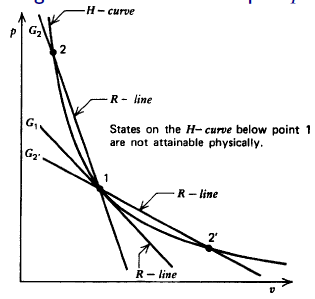
\includegraphics[scale=0.5]{ch7/chap710.png}
\caption*{Figure 7.11}
\end{center}
\end{figure}


Figure 7.11 shows the intersection between the Hugoniot curve and Rayleigh lines in a p-v diagram (where Rayleigh lines are straight lines by definition). 

Let's consider several Rayleigh lines passing through the initial state 1. The line $G_1$ tangent to the Rayleigh line separates the lines of higher slope (such as $G_2$) that intersects the Hugoniot curve at a point of higher pressure (case 1), and the lines of lower slope (such as $G'_2$) that intersects the Hugoniot curve at a point of lower pressure (case 2). As shown before only the transformations from case 1 are possible. The case of the line $G_1$ marking the separation between the upper and lower branches of the Hugoniot curves correspond to sonic conditions at point 1. 

The upper branch, admissible, of the Hugoniot curve correspond to supersonic conditions at 1. And so, a shock wave can only appear in supersonic flows.
\\

Note: It can also be observed that an increase of entropy leads to a drop of the stagnation pressure. This explains why the stagnation pressure is used as a loss indicator in some application such as turbomachines for example.
\\

\textbf{Let's do a little recapitulation for the flow with a shock wave in a Laval (convergent-divergent) nozzle:}
\\

We have seen before learning about shock waves that there were no isentropic solutions in a Laval nozzle for a downstream pressure between subsonic solutions $c$ and saturated supersonic $d$ (cf. figure 7.6). 

Let's now suppose that a normal shock wave appears in the divergent in a given place. Rankine-Hugoniot relations allows us to calculate the conditions behind the shock, in particular the pressure and the Mach number. The flow being subsonic behind the shock, it decelerates in the rest of the divergent, and we can calculate its evolution by the theory of isentropic flow in a nozzle. We see that the outlet pressure is inferior to the one in case $c$. It is the case $h$ in figure 7.6. As a matter of fact, if the transformation trough the shock was isentropic, the pressure behind the shock would be identical to the one at $c$. But since there is a drop of the stagnation pressure through the shock, the pressure behind the shock is inferior, and therefore, all the pressure distribution downstream is inferior than the one in case c.
\\

Since the stagnation pressure drop increase with the Mach number ($M_1$) before the shock, it results that the outlet pressure decrease as the shock moves to the exit of the nozzle. For a given exit pressure, the position of the shock is unknown. We have to determine it by iterations. The extreme case (case $g$ in figure 7.6) is the one where the shock is located in the exit section.
\\

We can now calculate the flow in a nozzle for downstream pressures between the case $a$ and $g$. For a pressure inferior than the case $g$, the augmentation of pressure between the adapted pressure and the downstream pressure can take place only outside the nozzle with oblic shock waves (not seen in this course). Pratically, we observe that oblic shock waves climb back into the nozzle for pressure slightly below the pressure at point $g$.

\end{document}